\section{Les SiPM, un détecteur de lumière}
Au plus simple, un SiPM est un composant électronique qui permet de détecter de la lumière.

Un SiPM est une puce de silicium qui contrairement au processeur qui sont composés de transistors, est composé d'une multitude de photodiodes. Une photodiode est un composant électronique qui permet de convertir de la lumière en courant électrique. C'est notamment ce qui est à utiliser dans les cellules photovoltaïques des panneaux solaires. Ici, les photodiodes vont plutôt être optimisées pour détecter des photons que pour générer de l'électricité. 

En temps normal, une jonction p-n est un assemblage de deux matériaux semi-conducteurs qui agisse comme une diode (voir \cref{fig_pn_diode}). En choisissant judicieusement ses matériaux et en lui appliquant une tension dans son sens conventionnelle, on peut obtenir l'émission de lumière. C'est le principe de la LED. En revanche, si l’on applique une tension dans le sens inverse alors le courant ne peut plus circuler, car c'est une diode. Quand un photon d'une énergie suffisante vient frapper la jonction, il va libérer un électron qui va créer un courant électrique proportionnel au nombre de photons qui entre. C'est le principe de la photodiode.

Notre détecteur peut être plus sensible si nous augmentons la tension alors nous commençons à observer un phénomène d'avalanche. En effet, quand une paire électron-trou est créée, elle va accélérer dans le champ électrique et libéré d'autre paire électron-trou. C'est le principe du photodétecteur avalanche (APD)
(avalanche photodetector), mais nous arrivons rapidement a une limite~; à une certaine tension, dite la tension de claquage, la diode va se mettre a conduire dans le sens inverse. Dans ce cas, le photon que nous détecterons en premier créera un courant qui s'entretiendra tout seul. Pour empêcher cela, il faut donc limiter le courant du signal. Dans le cas des SiPM, cela est fait avec une résistance et une accumulatrice pour former ce qu'on appellera un SPAD (Single photon avalanche diode).

Dans un SiPM, nous allons relier en parallèle des centaines, voir des milliers de ces SPAD (voir \cref{fig_SiPM}). Ainsi, on augmente la surface de détection pour un photon. Actuellement, dans le commerce, la taille la plus grande de SiPM disponible est de 6*6~mm~\cite{site:sipm_vendor}. En couplant plusieurs SiPM en parallèle, on peut donc détecter des photons sur une surface plus grande.

\begin{figure}
    \centering
    % \begin{subfigure}{0.45\textwidth}
    %     \centering
    %     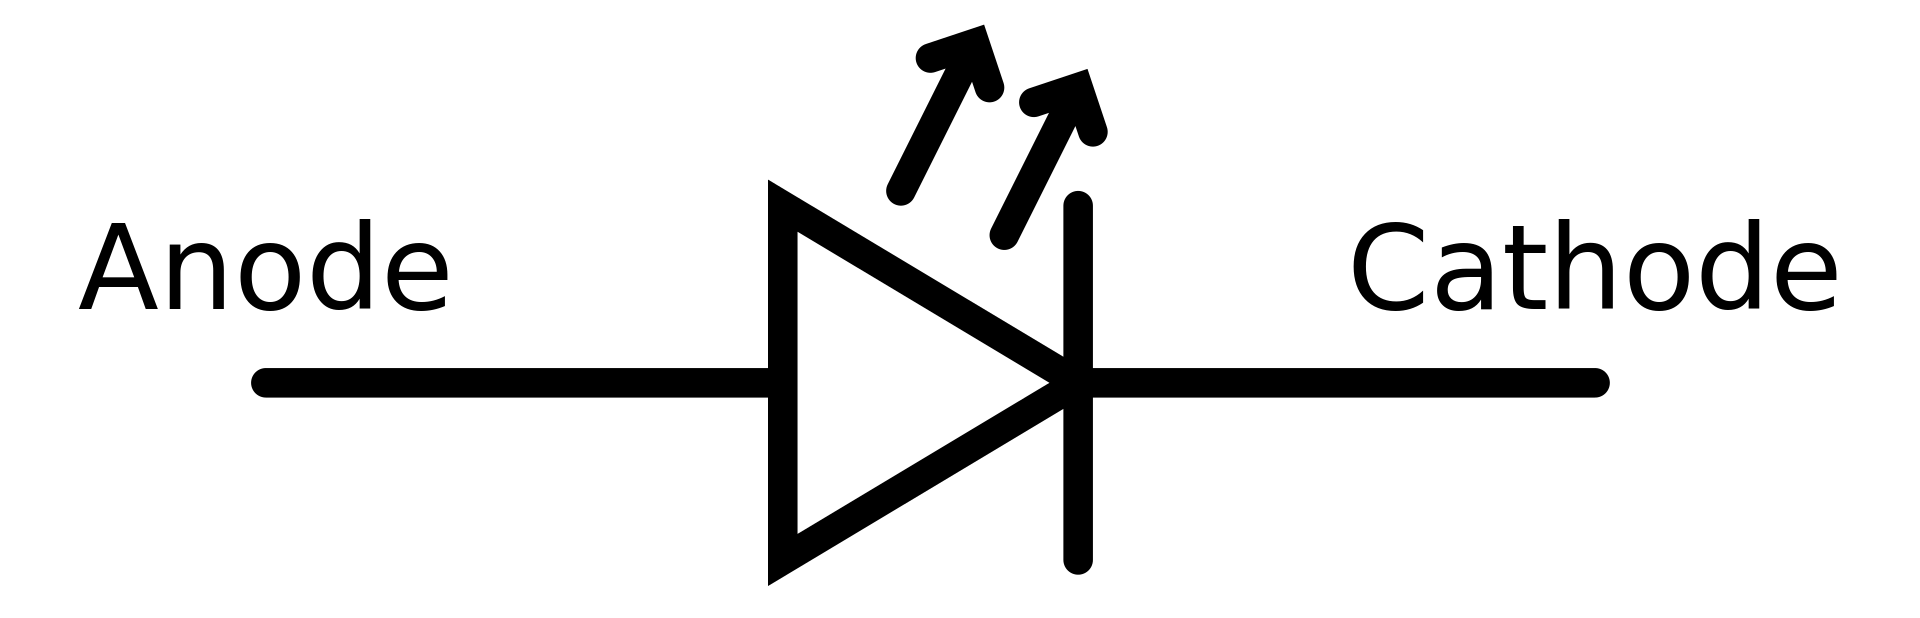
\includegraphics[width=\textwidth]{img/she/LED_symbol.svg.png}
    %     
    %     \caption{Source: \href{https://commons.wikimedia.org/wiki/File:LED_symbol.svg}{Omegatron}, \href{https://creativecommons.org/licenses/by-sa/3.0}{CC BY-SA 3.0}, via Wikimedia Commons}
    %     \label{fig_LED_elec_symbol}
    % \end{subfigure}
    % \begin{subfigure}{0.45\textwidth}
    %     \centering
    %     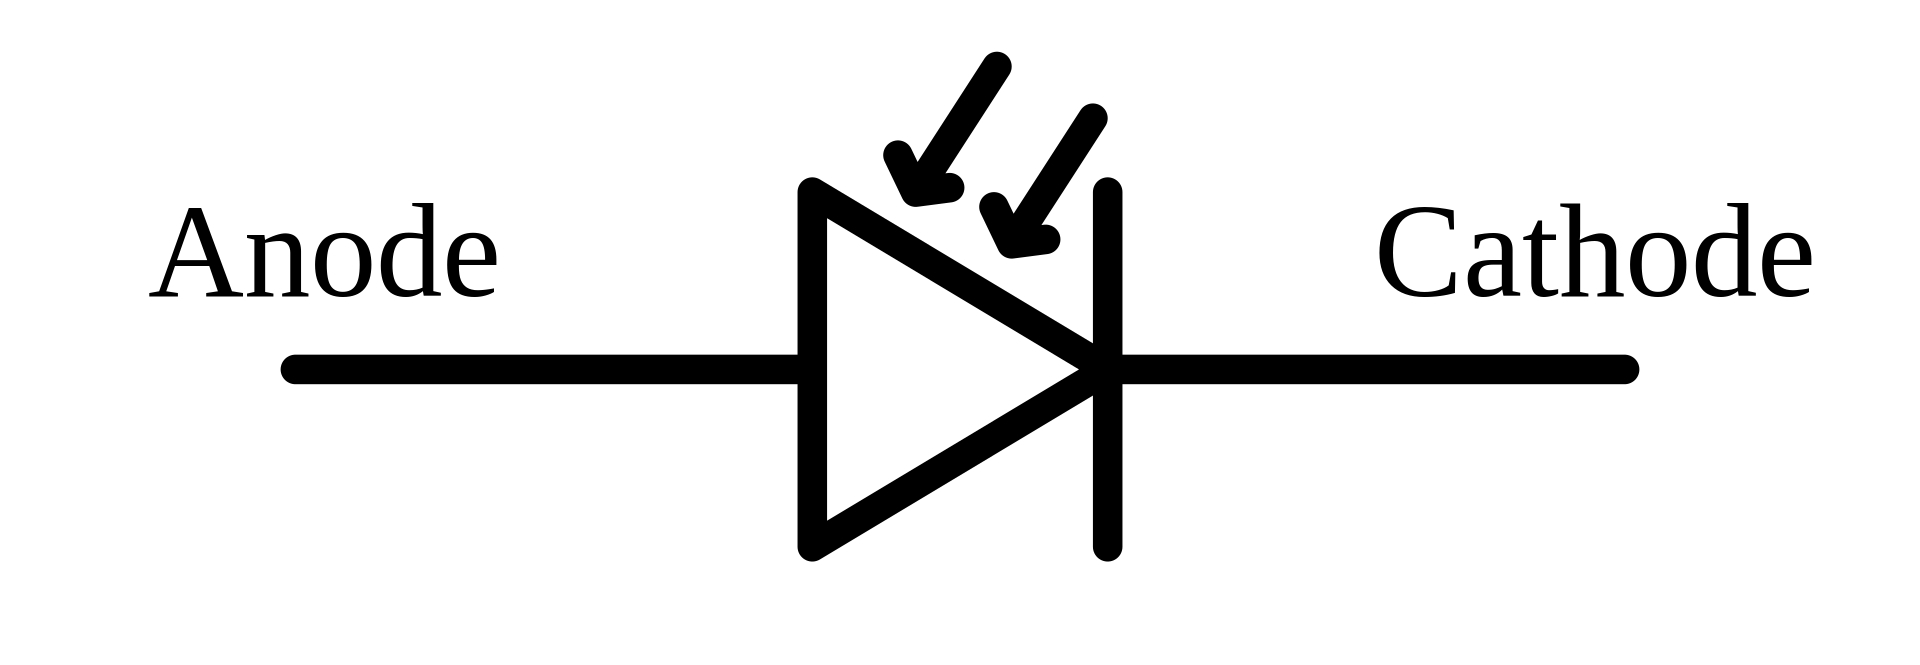
\includegraphics[width=0.85\textwidth]{img/she/Photodiode_symbol.svg.png}
    %     
    %     \caption{Source: \href{https://commons.wikimedia.org/wiki/File:Photodiode_symbol.svg}{Simone Biancolilla}, \href{https://creativecommons.org/licenses/by-sa/3.0}{CC BY-SA 3.0}, via Wikimedia Commons}
    %     \label{fig_photodiode_elec_symbol}
    % \end{subfigure}
    \begin{subfigure}[c]{0.45\textwidth}
        \centering
        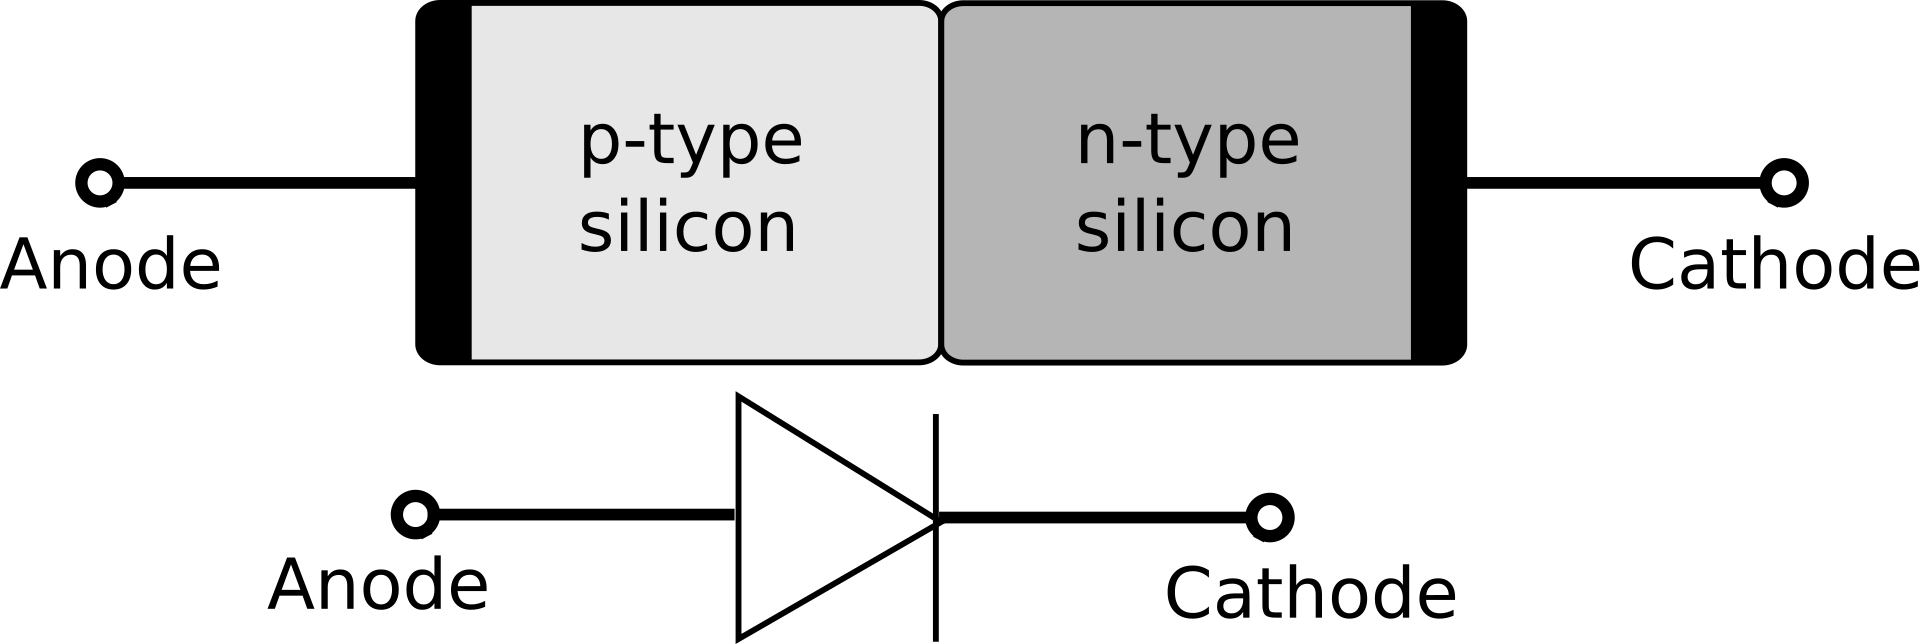
\includegraphics[trim= 0 -585 0 -585, width=0.85\textwidth]{img/she/1920px-PN_diode_with_electrical_symbol.svg.png}
        
        \caption{Schéma montrant l'équivalence entre une jonction P-N et une diode. Source~: \href{https://commons.wikimedia.org/wiki/File:PN_diode_with_electrical_symbol.svg}{Raffamaiden}, \href{https://creativecommons.org/licenses/by-sa/3.0}{CC BY-SA~3.0}, via Wikimedia Commons}
        \label{fig_pn_diode}
    \end{subfigure}
    \begin{subfigure}[c]{0.45\textwidth}
        \centering
        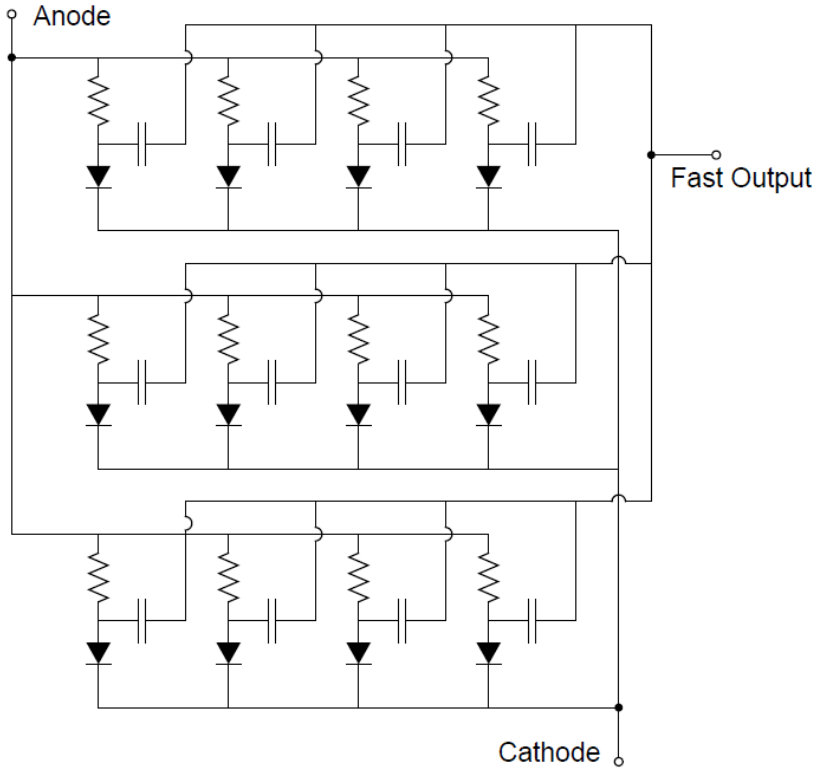
\includegraphics[width=0.85\textwidth]{img/she/SiPM_arithecture.png}
        
        \caption{Schéma d'un SiPM. Les diodes sont des diodes photoavalanche. On ne représente pas tous les modules. Source~: \href{https://websites.umich.edu/~ners580/ners-bioe_481/lectures/pdfs/2017-02-.pdf}{An Intro to SiPM, SensL}}
        \label{fig_SiPM}
    \end{subfigure}
    \caption[Composition d'un SiPM]{Composition d'un SiPM}
\end{figure}
